\section{Part B.  Self Instructing Database:}
\label{part_b}
\subsection{Overview:}
Any standard database has considerable large number of configuration knobs. Databases needs to be tweaked with proper configuration for running efficiently with different workloads and hardware resources. Tweaking database configuration knowbs needs a great level of expertise from database administrator (DBA) because optimal configuration varies with the type of worloads. Beside that even finding optimal knob configurations might involve trial and error process for a DBA (which restrits the search spaces for knobs). An auto-configuring database system or self intructing database is a desirable feature to demand from database companies.


Human database administrators rely on experience and intuition to configure it. DRL process mimick same learning strategies i.e. learn from mistakes and correctness to maximize future rewards. Keeping this in mind we can explore how DRL can provide a solution to automatic database tuning.


\subsection{Problem Formulation:}
Given a workload $\mathcal{W}$ (which is a serialized query profile DAG of execution task), with a knobs setting $\mathcal{C} = \{c_1,c_2,\ldots,c_{|\mathcal{C}|}\}$ a typical database outputs a log of metrics $\mathcal{M} = \{m_1,m_2,m_3,\ldots,m_{|\mathcal{M}|}\}$ as shown in Figure \ref{fig:database_01}.
The database keeps receiving workloads at some discrete interval of time and it runs with some configuration and outputs a metric log, which is also called a discrete time stochastic control process.

\begin{figure}[h]
	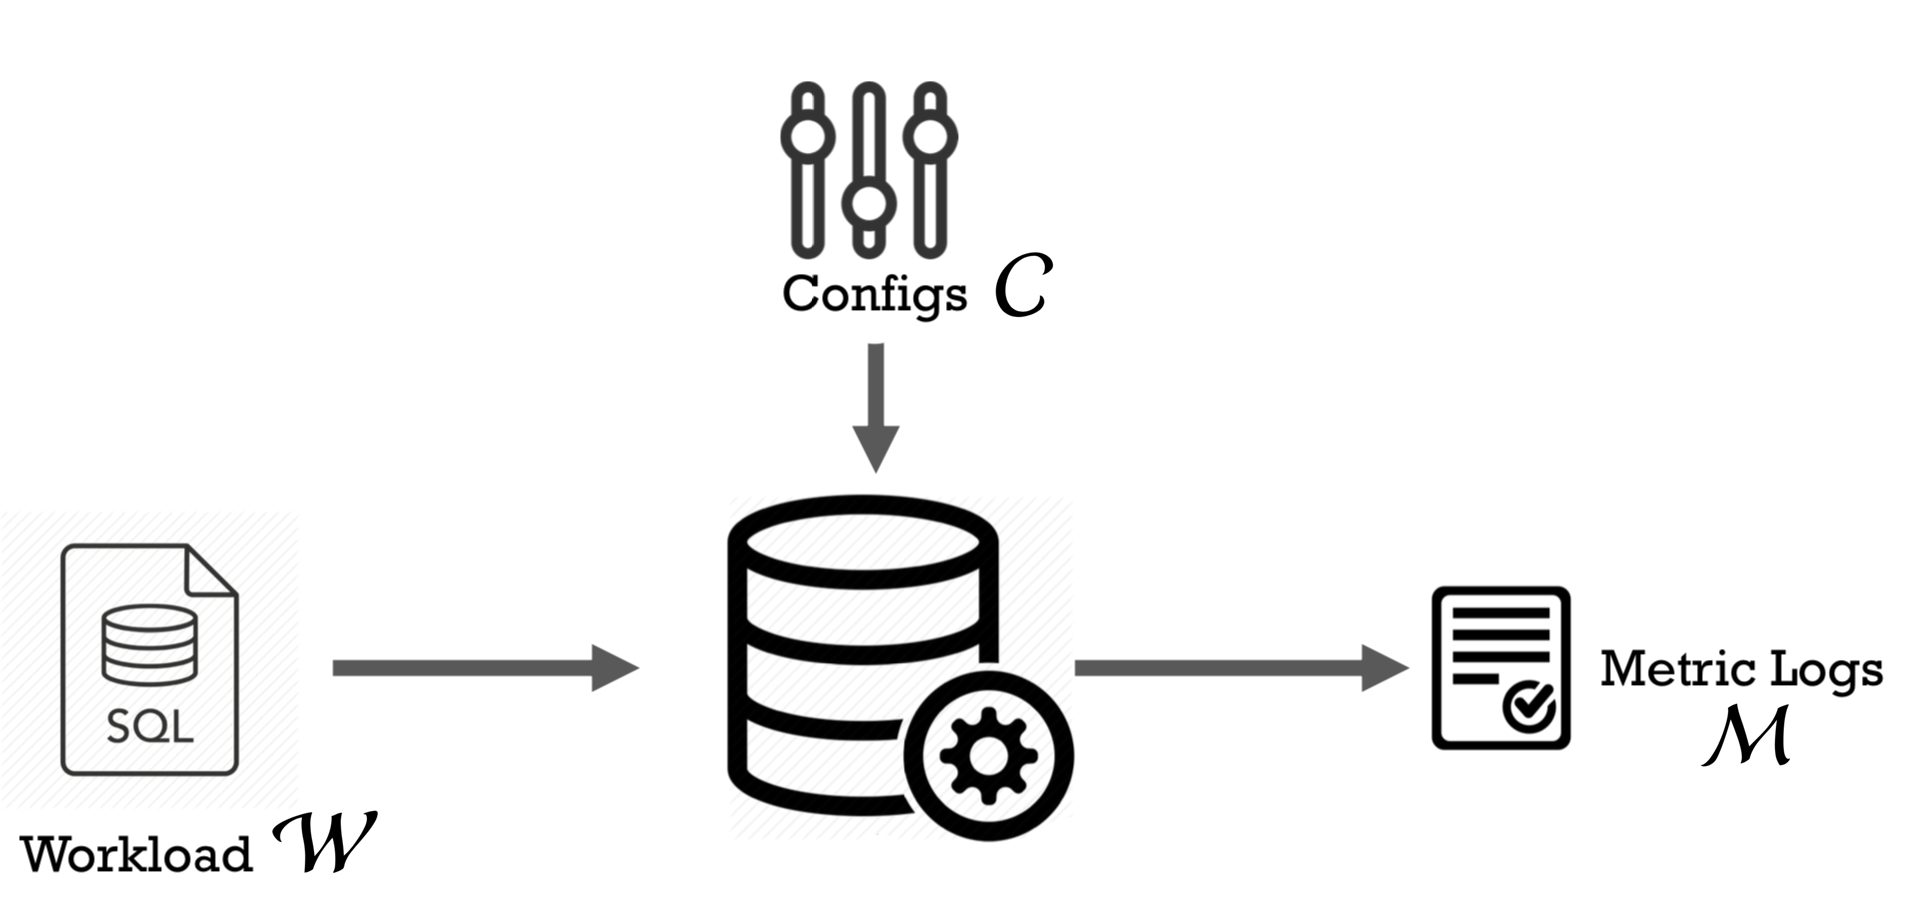
\includegraphics[width=0.9\linewidth ]{fig/database_01.png}
    \vspace{-2mm}
    \caption{A typical database system.}
    \label{fig:database_01}
\end{figure}


We can apply deep reinforcement learning to train a neural network in taking
over the database tuning process by optimizing configuration for observable database workload.
Essentially, we have to define a RL problem environment
consisting of the four following components to perform the learning as shown in Figure \ref{fig:database_agent}:


\textbf{1) Observable State:} This is also input to the neural network. This is typically the current workload in form of
query characteristics, for which the system should be optimised as well as the current state
of the configuration. Figure \ref{fig:database_agent} illustrates workload $\mathcal{W}_t$ is mapped to observation/state $\omega_t \in \Omega$ or $s_t \in  \mathcal{S}$ for time stamp $t$. (Note: $\omega_t = s_t$ in MPD)\\
\textit(Note: These notations are defined in Section \ref{formal_rl}).

\textbf{2) Actions:} An action is a bounded set of configuration $\mathcal{C}_t$ where each knobs can have a range of permissible values.
Changing the size of a database buffer is an example of action. Now we can represent $\mathcal{C}_t  \rightarrow a_t \in \mathcal{A}$.

\textbf{3) Reward:}
We map the metric $\mathcal{M}_t$ to rewards $r_t \in \mathcal{R}$. Since reward is a scalar function and metric $\mathcal{M}_t$ is a set of values representing the goodness and badness of database execution on workload $\mathcal{W}_t$, we need to apply some function $r_t = f(\mathcal{M}_t)$ to keep it simple. Later we will see an alternative approach where function $f$ is not needed with multi-agent DRL.

\textbf{4) Hyperparamters for Neural Network:}
This includes properties of
the neural network (e.g. number of hidden layers, number of nodes per layer) as well as
properties of the learning process like the number of iterations.




% We apply this process into a RL agent-database environment interaction process as shown in Figure \ref{fig:database_agent}.
% In this process, at each time step $t$ we map metric $\mathcal{M}_t$ to rewards $r_t$. Similarly, workload $\mathcal{W}_t$ is mapped to observation/state $\omega_t$ or $s_t$, and configuration $C_t$ is mapped to action $a_t$.



\begin{figure}[h]
  \vspace{-3mm}
	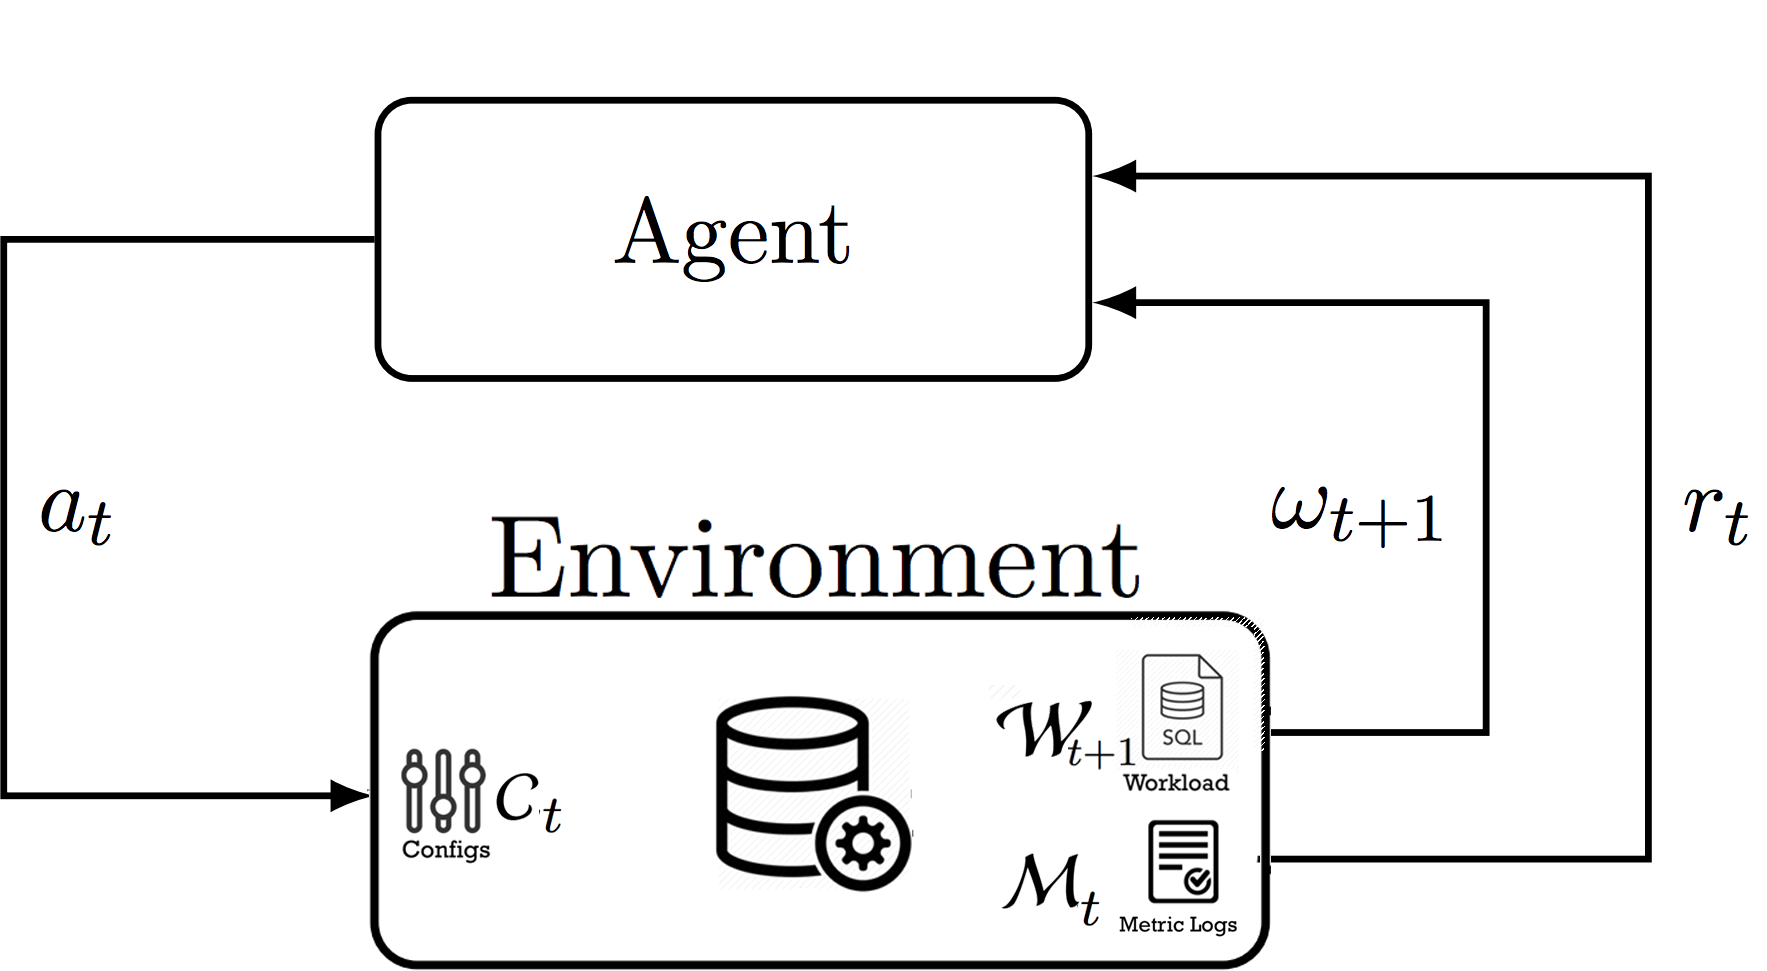
\includegraphics[width=\linewidth ]{fig/database_agent.png}
    \vspace{-5mm}
    \caption{RL Agent-Database Environment Interaction.}
    \label{fig:database_agent}
    \vspace{-5mm}
\end{figure}


\subsection*{Training and Prediction:}
With the high level components defined, now we will go through the workflow of learner.
Assuming the {\em neural network agent (NNA) } is configured with required hyperparamters, the learning process starts with time $t=0$.
First, a workload $\mathcal{W}_t = s_t$  is feed into {\em neural network agent} (NNA). Then, the NNA explore action set $\mathcal{A}$ to produce an action (configuration) $a_t = \mathcal{C}_t$. The database environment on receiving action configuration $\mathcal{C}_t$ executes workload $\mathcal{W}_t$ and returns with metrics $\mathcal{M}_t$. Some function $f: \mathcal{M}_t \rightarrow r_t \in \mathbb{R}$ converts metric to scalar reward. This process is repeated many times and agents either explore action set or exploit learned optimal action to predict next best configuration. The desired goal is to optimize maximum cumulative positive rewards.

An intuitive solution for choosing function $f: \mathcal{M}_t \rightarrow r_t \in \mathbb{R}$ is  through these steps:\\
\vspace{-4mm}
\begin{itemize}
  \item[-] negate all the metrics whose desired objective is to minimize, such that we now optimize for maximization.
  \item[-] normalize each metric $m_i \in \mathcal{M}_t$ with their satisfied range of operation.
  \item[-] rewards is sum  of normalized metrics.
\end{itemize}

To avoid the problem of choosing a function $f$, we can transform the problem to a {\em Multi-task Deep RL} problem.
Some hierarchical RL techniques also decompose tasks into subtasks, these methods then solve the subtasks
in a locally optimal way and then global optimality can be achieved by aggregating back together. Another approach is to try {\em Linear Temporal Logic} specification that enables an interleaving of subtasks to support global optimization \cite{icarte2018teaching}.
These techniques can help in avoiding selection of $f$ by considering specific set of metrics and optimize actions for it.


\paragraph{Model based/Model-free Agent:}
Model-free and model based both type of agent can be frutiful in this type of scenario. However model based approach needs more effort in design.
The advantage of model based approach is that it can learn strategies to trade-off exploration and eploitation to learn quickly.
But it is non-arguably plausible to choose gradient based methods because configurations knobs tend to have convex properties. 



%%% Local Variables:
%%% mode: latex
%%% TeX-master: "main"
%%% End:
